\documentclass[aspectratio=169,9pt]{beamer}

\usepackage{amsmath}
\usepackage{amssymb}
\usepackage{booktabs}
\usepackage{tabularx}
\usepackage{graphicx}
\usepackage{ragged2e}
\usepackage{xcolor}

\definecolor{eiBlue}{HTML}{1F4E79}
\definecolor{eiTeal}{HTML}{2F7E8A}
\definecolor{eiGray}{HTML}{4A5568}
\definecolor{eiLight}{HTML}{EEF4F8}

\usetheme{Madrid}
\usecolortheme{default}
\setbeamercolor{palette primary}{bg=eiBlue,fg=white}
\setbeamercolor{palette secondary}{bg=eiTeal,fg=white}
\setbeamercolor{frametitle}{bg=eiBlue,fg=white}
\setbeamercolor{title}{bg=eiBlue,fg=white}
\setbeamercolor{subtitle}{fg=white}
\setbeamercolor{block title}{bg=eiBlue,fg=white}
\setbeamercolor{block body}{bg=eiLight,fg=black}
\setbeamercolor{structure}{fg=eiBlue}
\setbeamertemplate{navigation symbols}{}
\setbeamertemplate{itemize items}[circle]
\setbeamertemplate{enumerate items}[default]

\newcommand{\exercise}[1]{\textbf{Ejercicio #1}}
\newcommand{\result}[1]{\textbf{\color{eiTeal}Resultado:} #1}
\newcommand{\unit}[1]{\,\mathrm{#1}}
\newcommand{\SN}{\mathrm{S/N}}
\newcommand{\GBW}{\mathrm{GBW}}
\newcommand{\CMRR}{\mathrm{CMRR}}

\title[Exhibición 02 - Grupo 1]{Exhibición 02: solución de ejercicios asignados}
\subtitle{Grupo 1 - Instrumentación electrónica}
\author[Ramírez, Estrada y Gallego]{\texorpdfstring{Martín Ramírez Espinosa\\Miguel Angel Estrada Ocampo\\Brayan Manuel Gallego Ocampo}{Martín Ramírez Espinosa, Miguel Angel Estrada Ocampo, Brayan Manuel Gallego Ocampo}}
\institute[Lab. Instrumentación Electrónica]{Laboratorio de Instrumentación Electrónica}
\date[28 de abril de 2026]{28 de abril de 2026}

\begin{document}

\begin{frame}
  \titlepage
\end{frame}

\begin{frame}{Asignación del grupo 1}
  \begin{columns}[T,onlytextwidth]
    \begin{column}{0.52\textwidth}
      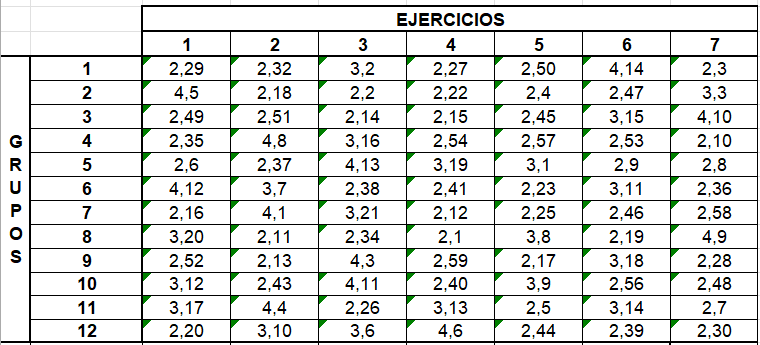
\includegraphics[width=0.98\linewidth]{../../exercises.png}
    \end{column}
    \begin{column}{0.44\textwidth}
      \begin{block}{Ejercicios de la primera fila}
        \centering
        \begin{tabular}{ccccccc}
          \toprule
          1 & 2 & 3 & 4 & 5 & 6 & 7\\
          \midrule
          2.29 & 2.32 & 3.2 & 2.27 & 2.50 & 4.14 & 2.3\\
          \bottomrule
        \end{tabular}
      \end{block}
      \vspace{0.4em}
      \justifying
      La presentación organiza cada problema con el mismo criterio: interpretación instrumental, modelo de error, cálculo y conclusión de diseño.
    \end{column}
  \end{columns}
\end{frame}

\begin{frame}{Mapa conceptual de la presentación}
  \begin{tabularx}{\textwidth}{@{}lX@{}}
    \toprule
    \textbf{Bloque} & \textbf{Idea dominante}\\
    \midrule
    2.3, 2.27, 2.29, 2.32, 2.50 & Limitaciones reales del amplificador operacional: saturación, ganancia finita, offset, polarización, ruido y ancho de banda.\\
    3.2 & Uso de un amplificador instrumental integrado para una señal diferencial de puente.\\
    4.14 & Compromiso entre ancho de banda, error de ganancia y filtrado de ruido en un sistema de dos etapas.\\
    \bottomrule
  \end{tabularx}
\end{frame}

\begin{frame}{\exercise{2.29}: fotodiodo y amplificación de corriente}
  \begin{block}{Planteamiento}
    Un fotodiodo se modela como fuente de corriente y se desea obtener una salida de fondo de escala de \(4\unit{V}\) mediante una etapa transimpedancia seguida de una etapa inversora. El operacional se alimenta a \(\pm 5\unit{V}\) y sus datos relevantes son los de la Tabla 2.6 del libro.
  \end{block}

  \begin{columns}[T,onlytextwidth]
    \begin{column}{0.48\textwidth}
      \begin{itemize}
        \item Primera etapa: \(R_F=10\unit{M\Omega}\).
        \item Segunda etapa: \(R_F=40\unit{k\Omega}\), \(R_{in}=100\unit{\Omega}\).
        \item Ganancia efectiva de la segunda etapa:
        \[
          A_2 = 1+\frac{40\unit{k\Omega}}{100\unit{\Omega}}=401 .
        \]
      \end{itemize}
    \end{column}
    \begin{column}{0.48\textwidth}
      \begin{itemize}
        \item Peor caso térmico: \(0\) a \(60^\circ\mathrm{C}\).
        \item Máxima separación respecto a \(25^\circ\mathrm{C}\):
        \[
          \Delta T=35^\circ\mathrm{C}.
        \]
        \item Por tanto:
        \[
          v_{io,\max}=65\unit{\mu V}+2\unit{\mu V/^\circ C}(35)=135\unit{\mu V}.
        \]
      \end{itemize}
    \end{column}
  \end{columns}
\end{frame}

\begin{frame}{\exercise{2.29}: error máximo sin compensación}
  \begin{block}{Corriente de polarización en el peor caso}
    \[
      I_{B,\max}=130\unit{pA}+15\unit{pA/^\circ C}(35)=655\unit{pA}.
    \]
  \end{block}

  \begin{columns}[T,onlytextwidth]
    \begin{column}{0.48\textwidth}
      Primera etapa:
      \[
        R_{Th-}=10\unit{M\Omega},\qquad R_{Th+}=0 .
      \]
      Con los términos de offset, polarización y corriente de offset:
      \[
        v_{oo1}\simeq 7.6\unit{mV}.
      \]
    \end{column}
    \begin{column}{0.48\textwidth}
      Segunda etapa:
      \[
        R_{Th-}=100\parallel 40\unit{k}\simeq 99.8\unit{\Omega}.
      \]
      El offset de salida propio de esta etapa es:
      \[
        v_{oo2}\simeq 54\unit{mV}.
      \]
    \end{column}
  \end{columns}

  \[
    v_{oo}=401v_{oo1}+v_{oo2}\simeq 3.1\unit{V}.
  \]

  \result{el error de continua es muy alto y puede llevar la salida a saturación cuando se suma a la señal útil.}
\end{frame}

\begin{frame}[shrink=8]{\exercise{2.29}: compensación y reajuste}
  \begin{block}{Compensación de corriente de polarización}
    Si se coloca una resistencia de compensación de \(10\unit{M\Omega}\) en la entrada no inversora de la primera etapa, se cancela el término dominante asociado a la corriente de polarización. En ese caso:
    \[
      v_{oo1}\simeq 1.1\unit{mV},\qquad
      v_{oo}\simeq 495.1\unit{mV}.
    \]
  \end{block}

  \begin{block}{Ajuste de offset}
    El ajuste útil debe actuar sobre la primera etapa, porque su error queda multiplicado por la ganancia de la segunda. Tras ajustar a \(25^\circ\mathrm{C}\), domina la deriva:
    \[
      v_{oo}\simeq 82+0.16t\quad [\unit{mV}],
    \]
    donde \(t\) está en meses.
  \end{block}

  \[
    0.20(82\unit{mV})=16.4\unit{mV}
    \quad\Rightarrow\quad
    t\simeq 100\ \text{meses}.
  \]

  \result{conviene compensar la primera etapa y reajustar aproximadamente cada ocho años si se admite un incremento máximo del 20\%.}
\end{frame}

\begin{frame}{\exercise{2.32}: etapa inversora con OPA177F}
  \begin{block}{Planteamiento}
    Se implementa una etapa inversora con \(R_{in}=1\unit{k\Omega}\) y \(R_F=200\unit{k\Omega}\), usando el OPA177F. La entrada tiene fondo de escala de \(20\unit{mV}\) y las resistencias son de tolerancia \(0.1\%\).
  \end{block}

  \begin{columns}[T,onlytextwidth]
    \begin{column}{0.47\textwidth}
      Ganancia ideal:
      \[
        A_v=-\frac{200\unit{k\Omega}}{1\unit{k\Omega}}=-200.
      \]
      Fondo de escala:
      \[
        V_{o,FS}=200(20\unit{mV})=4\unit{V}.
      \]
    \end{column}
    \begin{column}{0.49\textwidth}
      La evaluación separa tres fuentes:
      \begin{enumerate}
        \item tolerancia de resistencias,
        \item ganancia diferencial finita,
        \item offset e intensidades de entrada.
      \end{enumerate}
    \end{column}
  \end{columns}
\end{frame}

\begin{frame}[shrink=25]{\exercise{2.32}: suma de errores}
  \begin{block}{Resistencias y ganancia finita}
    La tolerancia de dos resistencias en cociente introduce, en peor caso, el doble de la tolerancia:
    \[
      \varepsilon_R \simeq 0.2\%.
    \]
    Con la ganancia diferencial mínima del OPA177F, el error de ganancia finita es aproximadamente:
    \[
      \varepsilon_{A_d}\simeq 0.005\%.
    \]
  \end{block}

  \begin{block}{Offset}
    Para \(R_{Th-}=1\unit{k}\parallel 200\unit{k}\simeq 995\unit{\Omega}\), el offset máximo de salida es:
    \[
      v_{oo}\simeq 5.6\unit{mV}.
    \]
    Como el fondo de escala es \(4\unit{V}\):
    \[
      \varepsilon_{off}=\frac{5.6\unit{mV}}{4\unit{V}}\cdot100\simeq 0.14\%.
    \]
  \end{block}

  \[
    \varepsilon_T\simeq 0.2+0.005+0.14=0.34\%.
  \]

  \result{la tolerancia resistiva domina; reducir simplemente el valor absoluto de las resistencias apenas mejora el error principal.}
\end{frame}

\begin{frame}{\exercise{3.2}: puente de temperatura con AD620}
  \begin{block}{Planteamiento}
    La salida diferencial del puente varía linealmente de \(0\unit{mV}\) a \(10\unit{mV}\) entre \(30^\circ\mathrm{C}\) y \(50^\circ\mathrm{C}\). Se requiere una salida entre \(0\unit{V}\) y \(5\unit{V}\), con modo común continuo de \(150\unit{mV}\), usando un AD620.
  \end{block}

  \begin{columns}[T,onlytextwidth]
    \begin{column}{0.48\textwidth}
      Ganancia requerida:
      \[
        G=\frac{5\unit{V}}{10\unit{mV}}=500.
      \]
      Para el AD620:
      \[
        R_G=\frac{49.4\unit{k\Omega}}{G-1}\simeq 100\unit{\Omega}.
      \]
    \end{column}
    \begin{column}{0.48\textwidth}
      Con salida que debe llegar a \(0\unit{V}\), no se debe alimentar como dispositivo de simple alimentación si no es rail-to-rail. Se adopta alimentación simétrica:
      \[
        V_S=\pm 12\unit{V}.
      \]
    \end{column}
  \end{columns}
\end{frame}

\begin{frame}[shrink=20]{\exercise{3.2}: error máximo en temperatura}
  \begin{block}{Contribuciones principales}
    \[
      \varepsilon_G\simeq 0.48\%,\qquad
      v_{off,out}=50\unit{\mu V}\cdot 500=25\unit{mV}.
    \]
    El offset representa:
    \[
      \varepsilon_{off}=\frac{25\unit{mV}}{5\unit{V}}\cdot100=0.5\%.
    \]
  \end{block}

  \begin{block}{Modo común}
    Con \(\CMRR\simeq 130\unit{dB}=3.16\cdot 10^6\):
    \[
      v_{oc}=\frac{150\unit{mV}}{3.16\cdot10^6}\simeq 47\unit{nV},
    \]
    que es despreciable frente a \(5\unit{V}\).
  \end{block}

  \[
    \varepsilon_T\simeq 0.48+0.5=0.98\%.
  \]
  Sobre un intervalo de \(20^\circ\mathrm{C}\):
  \[
    \Delta T_{\max}=0.0098(20^\circ\mathrm{C})\simeq 0.196^\circ\mathrm{C}.
  \]

  \result{el error esperado es del orden de \(0.2^\circ\mathrm{C}\), dominado por ganancia y offset.}
\end{frame}

\begin{frame}{\exercise{2.27}: señal débil entre 10 Hz y 1 kHz}
  \begin{block}{Planteamiento}
    Se debe amplificar una señal de baja amplitud hasta \(10\unit{V}\) usando operacionales. El diseño de referencia usa dos etapas de ganancia 100 para evitar exigir toda la ganancia a una sola etapa.
  \end{block}

  \begin{columns}[T,onlytextwidth]
    \begin{column}{0.48\textwidth}
      Ganancia por etapa:
      \[
        A_1=A_2=100,\qquad A_T=10^4.
      \]
      Una elección práctica:
      \[
        R_1=1\unit{k\Omega},\qquad R_2=99\unit{k\Omega}.
      \]
    \end{column}
    \begin{column}{0.48\textwidth}
      Alimentación:
      \[
        V_o=10\unit{V}_{\text{amplitud}},
      \]
      por lo que \(\pm 12\unit{V}\) permite margen de excursión para operacionales no rail-to-rail.
    \end{column}
  \end{columns}
\end{frame}

\begin{frame}{\exercise{2.27}: offset de dos etapas}
  \begin{block}{Datos del operacional}
    \[
      v_{io}=80\unit{\mu V},\quad I_B=1\unit{nA},\quad I_{io}=600\unit{pA}.
    \]
    En cada etapa:
    \[
      R_{Th+}=R_{Th-}=1\unit{k}\parallel 99\unit{k}\simeq 990\unit{\Omega}.
    \]
  \end{block}

  \[
    v_{oo1}=v_{oo2}\simeq
    100\left(80\unit{\mu V}+\frac{990+990}{2}600\unit{pA}\right)
    =8.13\unit{mV}.
  \]

  \[
    v_{oo}=100v_{oo1}+v_{oo2}\simeq 821\unit{mV}.
  \]

  \[
    \varepsilon_{off}=\frac{0.821\unit{V}}{10\unit{V}}\cdot100\simeq 8.21\%.
  \]

  \result{la salida conserva la forma senoidal, pero aparece desplazada por una continua de aproximadamente \(0.82\unit{V}\).}
\end{frame}

\begin{frame}{\exercise{2.27}: mejora del comportamiento}
  \begin{block}{Separar señal alterna y continua}
    Como la banda útil comienza en \(10\unit{Hz}\), puede insertarse un acoplamiento de alta frecuencia de paso entre etapas para bloquear el offset de la primera etapa. Si se fija \(f_c\) dos décadas por debajo:
    \[
      f_c \approx 0.1\unit{Hz},\qquad RC=\frac{1}{2\pi f_c}\approx 1.6\unit{s}.
    \]
  \end{block}

  \begin{block}{Redistribución de ganancia}
    Otra mejora consiste en aumentar la ganancia de la primera etapa y reducir la de la segunda, por ejemplo:
    \[
      A_1=1000,\qquad A_2=10.
    \]
    Así, el offset de la segunda etapa se amplifica menos y el error final se aproxima a \(0.1\%\), siempre que la ganancia diferencial del operacional sea suficiente.
  \end{block}

  \result{la solución práctica requiere bloquear la continua de la primera etapa y revisar la distribución de ganancia; el problema no se resuelve sólo con que el circuito amplifique.}
\end{frame}

\begin{frame}[shrink=8]{\exercise{2.50}: sistema diferencial + etapa no inversora}
  \begin{block}{Planteamiento}
    El sistema tiene dos etapas: una diferencial de \(40\unit{dB}\) y una no inversora de ganancia 10. El operacional de ambas etapas presenta \(\GBW=100\unit{MHz}\). La señal diferencial útil va de \(100\unit{Hz}\) a \(10\unit{kHz}\), con amplitud máxima \(2\unit{mV}\), ruido de entrada y un modo común de \(2\unit{V}\) a \(50\unit{Hz}\).
  \end{block}

  \[
    A_1=100,\qquad A_2=10,\qquad A_T=1000.
  \]

  \begin{block}{Ancho de banda para error menor que 1\%}
    La etapa de mayor ganancia limita la respuesta. Con \(A_1=100\), su frecuencia de corte a 3 dB es:
    \[
      f_{3dB}=\frac{100\unit{MHz}}{100}=1\unit{MHz}.
    \]
    Para que la ganancia caiga sólo un 1\%:
    \[
      99=\frac{100}{\sqrt{1+(f/1\unit{MHz})^2}}
      \Rightarrow f\simeq 22.7\unit{kHz}.
    \]
  \end{block}
\end{frame}

\begin{frame}[shrink=20]{\exercise{2.50}: error de ganancia y S/N}
  \begin{block}{Error máximo de ganancia}
    En la máxima frecuencia útil, los errores relativos de las dos etapas se suman aproximadamente:
    \[
      G_{1,\mathrm{real}}\simeq 99.00,\qquad
      G_{2,\mathrm{real}}\simeq 9.990.
    \]
    Por tanto:
    \[
      \varepsilon_G\simeq 1.1\%.
    \]
  \end{block}

  \begin{block}{Relación señal a ruido}
    Al sumar cuadráticamente ruido resistivo, ruido del operacional y el efecto del modo común, el ruido equivalente de salida queda en el orden de:
    \[
      v_{N,out}\simeq 10.4\unit{mV}.
    \]
    La señal de salida de amplitud \(2\unit{V}\) tiene valor eficaz \(2/\sqrt{2}\unit{V}\):
    \[
      \SN=20\log_{10}\left(\frac{2/\sqrt{2}}{10.4\unit{mV}}\right)\simeq 42.7\unit{dB}.
    \]
  \end{block}

  \result{el ancho de banda cumple la señal útil, pero el ruido y el modo común reducen de forma importante la calidad de medida.}
\end{frame}

\begin{frame}[shrink=8]{\exercise{4.14}: dos etapas con THS4304}
  \begin{block}{Planteamiento}
    Un amplificador emplea dos etapas iguales de ganancia 100 con el THS4304. Se pide el ancho de banda compatible con un error máximo de ganancia de \(0.1\%\) y después un filtro que mejore la relación \(\SN\) sin reducir la ganancia más de \(0.05\%\) dentro de esa banda.
  \end{block}

  \begin{columns}[T,onlytextwidth]
    \begin{column}{0.48\textwidth}
      Para \(G>10\), el fabricante da:
      \[
        \GBW\simeq 870\unit{MHz}.
      \]
      Por etapa:
      \[
        f_p\simeq \frac{870\unit{MHz}}{100}=8.7\unit{MHz}.
      \]
    \end{column}
    \begin{column}{0.48\textwidth}
      Con dos polos iguales:
      \[
        |G(j\omega)|=
        \frac{10^4}{1+\left(\omega/5.5\cdot10^7\right)^2}.
      \]
    \end{column}
  \end{columns}

  \[
    9990=\frac{10^4}{1+\left(\omega/5.5\cdot10^7\right)^2}
    \Rightarrow
    \omega\simeq 1.7\unit{Mrad/s}.
  \]

  \result{\(f_{\max}\simeq 277\unit{kHz}\) para limitar la pérdida de ganancia al \(0.1\%\).}
\end{frame}

\begin{frame}[shrink=10]{\exercise{4.14}: filtrado y relación S/N}
  \begin{block}{Relación S/N sin filtro adicional}
    Considerando ruido térmico de resistencias y ruido blanco del THS4304, el ruido de salida se aproxima a:
    \[
      v_{N,out}\simeq 83\unit{mV}.
    \]
    Con el margen de salida disponible, la señal eficaz máxima es aproximadamente \(0.92\unit{V}\):
    \[
      \SN\simeq 20\log_{10}\left(\frac{0.92}{0.083}\right)=20.9\unit{dB}.
    \]
  \end{block}

  \begin{block}{Filtro pasa bajo}
    Un Butterworth de segundo orden exige una \(f_c\) tan alta que apenas reduce ruido. Con cuarto orden se obtiene \(f_c\simeq 1.9\unit{MHz}\) y:
    \[
      v_N\simeq 43\unit{mV},\qquad \SN\simeq 26.6\unit{dB}.
    \]
    Con sexto orden:
    \[
      f_c\simeq 980\unit{kHz},\qquad v_N\simeq 31\unit{mV},\qquad \SN\simeq 29.5\unit{dB}.
    \]
  \end{block}

  \result{el filtro mejora la S/N, pero la restricción de ganancia en banda impide una mejora grande.}
\end{frame}

\begin{frame}{\exercise{2.3}: alimentación del operacional para un A/D}
  \begin{block}{Planteamiento}
    Un sensor entrega una señal alterna máxima de \(10\unit{mV}\) que debe acondicionarse para un convertidor A/D con referencias estables de \(0\unit{V}\) y \(4.096\unit{V}\). Se debe seleccionar la alimentación del operacional.
  \end{block}

  \begin{columns}[T,onlytextwidth]
    \begin{column}{0.48\textwidth}
      Para aprovechar todos los bits del convertidor:
      \[
        V_o \in [0,4.096]\unit{V}.
      \]
      La señal alterna debe amplificarse y desplazarse para quedar centrada dentro del intervalo de conversión.
    \end{column}
    \begin{column}{0.48\textwidth}
      Con alimentación simple aparecen dos problemas:
      \begin{itemize}
        \item la salida no llega exactamente a \(0\unit{V}\) si el operacional no es rail-to-rail;
        \item la entrada puede no admitir tensiones próximas o inferiores a masa.
      \end{itemize}
    \end{column}
  \end{columns}
\end{frame}

\begin{frame}{\exercise{2.3}: criterio de selección}
  \begin{block}{Solución de diseño}
    La opción robusta es usar alimentación simétrica. Si el operacional es input/output rail-to-rail, \(\pm 5\unit{V}\) puede ser suficiente para cubrir \(0\) a \(4.096\unit{V}\). Para un operacional convencional, \(\pm 12\unit{V}\) da margen de entrada y de salida sin saturar cerca de los rieles.
  \end{block}

  \begin{block}{Conclusión instrumental}
    No basta con calcular la ganancia. La alimentación debe garantizar simultáneamente:
    \begin{enumerate}
      \item rango de modo común admisible en la entrada,
      \item excursión de salida compatible con el A/D,
      \item ausencia de saturación en los extremos \(0\unit{V}\) y \(4.096\unit{V}\),
      \item preservación del margen dinámico del convertidor.
    \end{enumerate}
  \end{block}

  \result{se recomienda alimentación doble; \(\pm 12\unit{V}\) es la selección conservadora si no se especifica un operacional rail-to-rail.}
\end{frame}

\begin{frame}{Conclusiones generales}
  \begin{itemize}
    \item En instrumentación, el error real rara vez depende de una sola causa; debe separarse en ganancia, offset, polarización, modo común, ruido y ancho de banda.
    \item Las primeras etapas son críticas porque sus errores se amplifican por todas las etapas posteriores.
    \item La reducción de ruido mediante filtros está limitada por la planitud de ganancia exigida en la banda útil.
    \item La alimentación del operacional forma parte del diseño, no es un detalle posterior: condiciona saturación, modo común y rango de salida.
    \item Para señales pequeñas, los ajustes de offset y la selección de topología suelen ser tan importantes como la ganancia nominal.
  \end{itemize}
\end{frame}

\begin{frame}{Resumen numérico}
  \small
  \begin{tabularx}{\textwidth}{@{}lXl@{}}
    \toprule
    \textbf{Ej.} & \textbf{Resultado principal} & \textbf{Decisión}\\
    \midrule
    2.29 & Offset sin compensar \(\approx 3.1\unit{V}\); con compensación \(\approx 495\unit{mV}\). & Compensar primera etapa y reajustar.\\
    2.32 & Error total \(\approx 0.34\%\). & Tolerancias mejores antes que resistencias menores.\\
    3.2 & Error de temperatura \(\approx 0.196^\circ\mathrm{C}\). & AD620 con \(G=500\), \(R_G\approx100\unit{\Omega}\).\\
    2.27 & Offset de salida \(\approx 821\unit{mV}\). & Bloquear continua y redistribuir ganancia.\\
    2.50 & Banda a 1\% \(\approx 22.7\unit{kHz}\); \(\SN\approx42.7\unit{dB}\). & Ruido y modo común son limitantes.\\
    4.14 & Banda a 0.1\% \(\approx277\unit{kHz}\); filtro 6o orden: \(\SN\approx29.5\unit{dB}\). & Mejora limitada por planitud.\\
    2.3 & Alimentación doble recomendada. & \(\pm12\unit{V}\) si no es rail-to-rail.\\
    \bottomrule
  \end{tabularx}
\end{frame}

\end{document}
